\documentclass[a4paper, 10pt]{article}
    \usepackage[subpreambles=true]{standalone}
    \usepackage[english, american, british]{babel}
    \usepackage[utf8]{inputenc}
    \usepackage[T1]{fontenc}
    \usepackage{hyphenat}
    \hyphenation{Mathe-matik wieder-gewinnen}
    \usepackage{amsmath}
    \usepackage{import}
    \usepackage{tabularx}
    \usepackage{graphicx}
    \usepackage[margin=2cm ]{geometry}

    \title{Einführung in die Softwaretechnik 2018 \\ Sheet 03}
    \author{Maximilian Frühauf}

\begin{document}
\maketitle
\begin{enumerate}
    \item 
    Functional Requirements for the Bumpers Game:
    \begin{enumerate}
        \item Start Game
        \item Stop Game
        \item Play Music
        \item Steer Car
        \item Choose Car Type
        \item Choose Collision Type
        \item Notify Player
        \item Crash Car
        \item Play Crash Sound
    \end{enumerate}

    \item 
    Quality Requirements for the Bumpers Game:

    Usability:
    \begin{itemize}
        \item The types of cars should be differentiable by the player.
        \item The Music should not distract the player.
        \item The Crash sound should be played when two cars collide. Also it has to 
        be loud enough to be heard with the music in the background. 
    \end{itemize}
    Reliability:
    \begin{itemize}
        \item The Game can be restarted at any time.
        \item It should support multiple fast user inputs in succession, without crashing.
    \end{itemize}

    Performance:
    \begin{itemize}
        \item The game can support up to 20 cars simultaneously on the screen.
        \item Button click should be executed immediately.
    \end{itemize}

    Supportability:
    \begin{itemize}
        \item The game has to be modifiable by the developer to correct defects.
        \item It has to be runnable on multiple different Operating Systems.
    \end{itemize}

    \item 
    \underline{As-is Scenario:}

    The user starts the game and is presented with the game screen.
    To start the game he has to click the start game button in the upper left hand corner.
    Now the Non-Player-Cars are moving on the game board and the player can steer his own car 
    with a mouse click. Also some music is played.

    If two of the cars on the screen intersect with each other a crash occurs. Therefore one of the 
    two cars gets crunched, the other can continue driving.
    When the only car still driving, is the player car, he has won the game. If he gets crunched 
    while other cars are still moving he loses the game.

    Whenever the player achieves a win or loss he is notified of the event. Then the game stops and 
    he can restart again if he wishes to.

    \underline{Visionary Scenario:}
    
    The user starts the game and is presented with the game screen.
    To start the game he has to click the start game button in the upper left hand corner.
    Now the Non-Player-Cars are moving on the game board and the player can steer his own car 
    with a mouse click. Also some music is played.

    If two cars crash the larger one wins the crash. After the crash the winning car gets
    the size of the losing one added to itself and becomes larger. 
    When the player has crashed all other cars and is therefore the largest car on the screen he wins
    the game.

    Whenever the player achieves a win or loss he is notified of the event. Then the game stops and 
    he can restart again if he wishes to.

    \item 
    Textual Description of the Use Case Car crash:

    \begin{tabularx}{\linewidth}{ r X }
        \hline
        Use Case Name & Car Crash \\
        \hline
        Participating Actors & The player car and one non-player car \\
        \hline
        Entry Conditions & The game has started and the two cars intersect each other. \\
        \hline
        Flow of Events & 
        \begin{enumerate}
            \item Depending on the speed of the two cars a winner of the collision is chosen. This
            is the faster of the two cars.
            \item The loser car gets crunched.
            \item The crash sound is played.
            \item A notification is printed to the console if the player car was the loser in the collision. 
            Otherwise the NPC (non-player car) is crunched and the player continues driving in the arena.
        \end{enumerate}
        \\
        \hline
        Exit Conditions & If a winner of the collision has been determined the Condition is exited. \\
        \hline
        Special Requirements & 
        Because the Collision is based on the speed of the two cars involved the game has to be run for 
        a least on time step. This allows the velocities of all cars to be calculated.
         \\
        \hline
    \end{tabularx}
    \item Difference between \textbf{<<extends>>} and \textbf{<<includes>>}:

        The <<includes>> stereotype in a UML diagram describes functionality that 
        is common to multiple use cases and can therefore be factored out.
        This allows multiple different use cases to access the same functionality.

        The <<extends>> stereotype is used to separate functionality from a use case
        that is only rarely called but still has to be separate from the main use case.

        This difference can be seen in the \textit{Start Game} use case. Here the use case 
        \textit{choose car type} is connected with an <<extends>> relationship because the 
        player has the option to choose another car but is not forced to do so. 
        The use case \textit{play music} however is connected with an <<includes>> stereotype 
        because the music is always played once the car starts, but it can also be used by
        other use cases. 
    \item Difference between \textbf{aggregation} and \textbf{composition}:
        Aggregation is used to convey that one object consists of the parts of another object.

        Composition however is a specialization of Aggregation and also imposes that 
        the child object is dependant on the parent. Therefore if the parent is deleted, 
        the child object has to get deleted as well.

        This concept can be seen in the UML class diagram in the GameBoard class.
        Here the GameBoard consists of one player, modeled by aggregation.
        The connection to the GameBoardUI class however is modeled as Composition, 
        because the GameBoardUI cannot exist on it's own. The parent of GameBoard is needed to 
        to use the GameBoardUI class.

        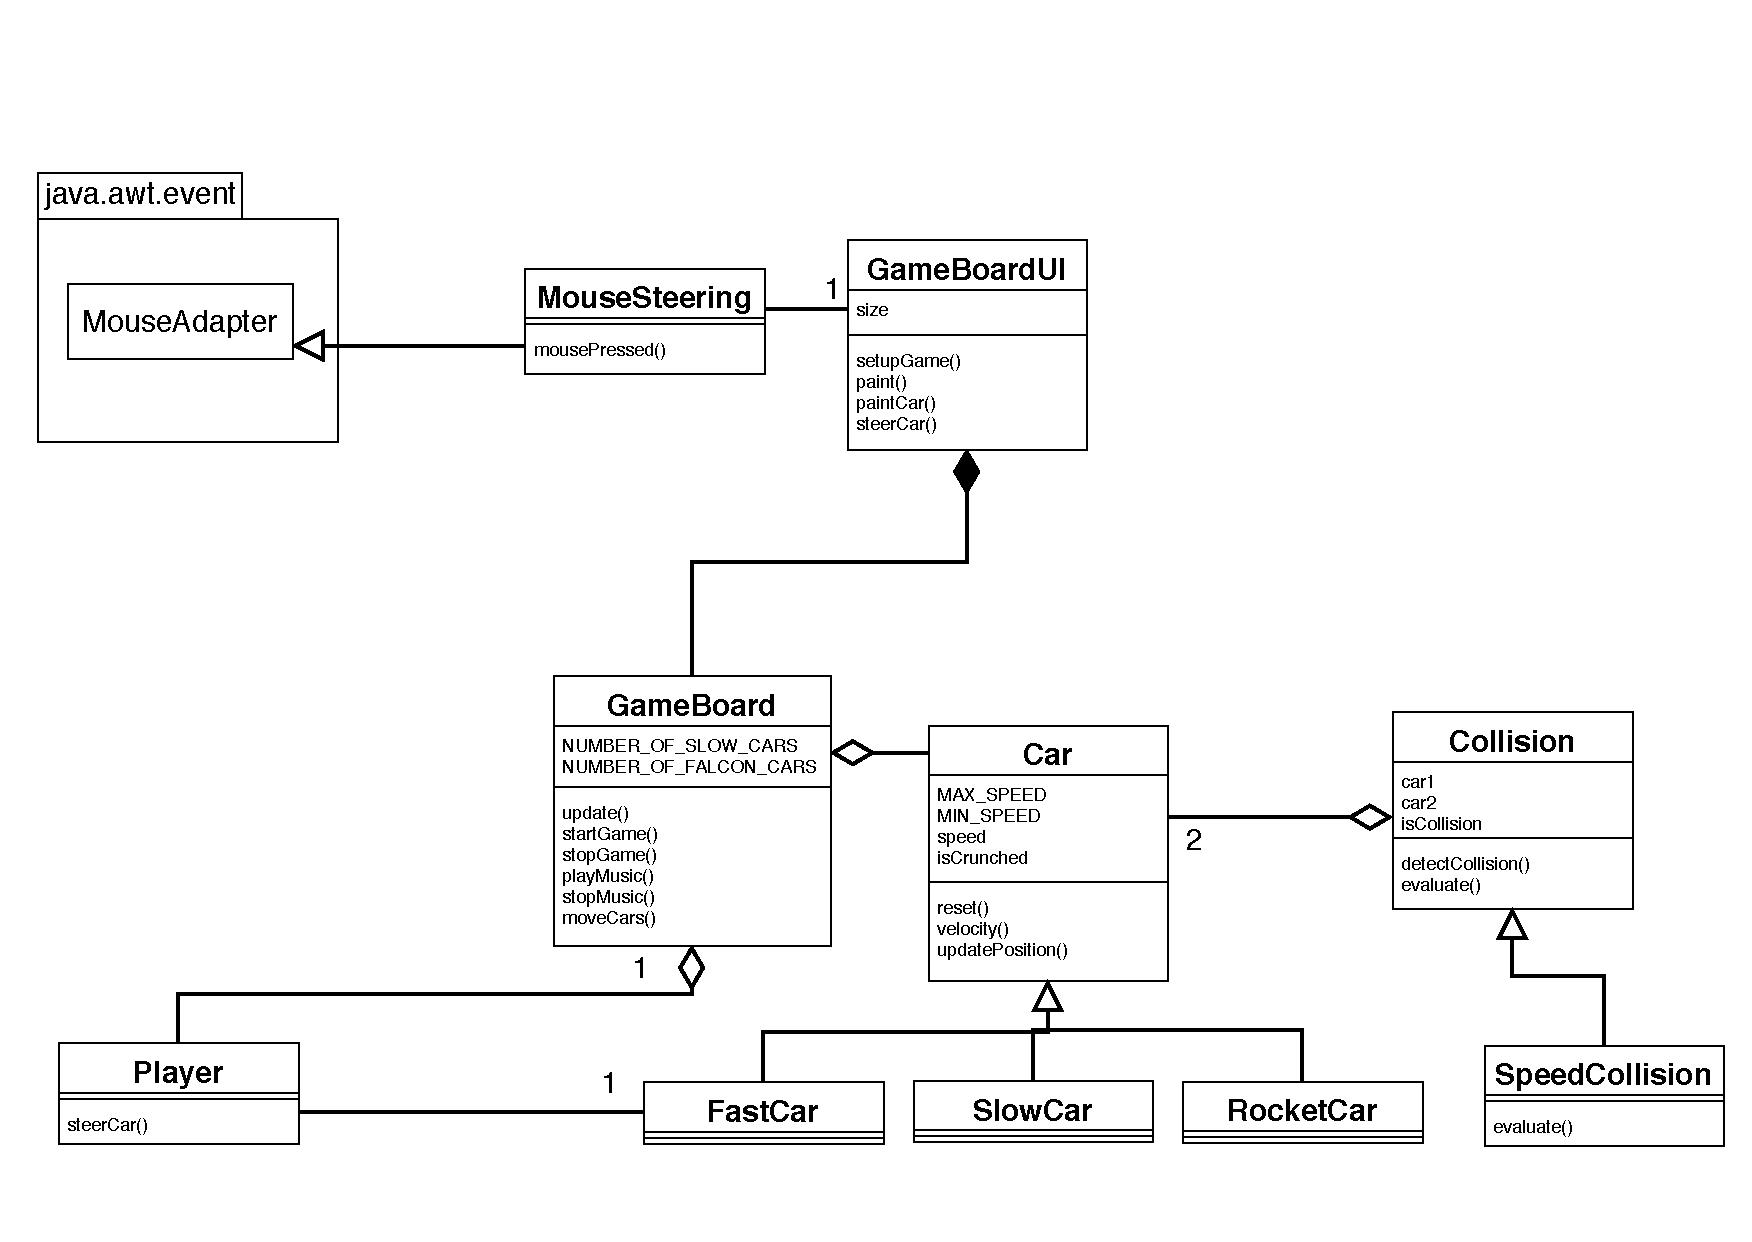
\includegraphics[width=10cm] {../sheet02/object_model.pdf}

\end{enumerate}

\end{document}